\section{Trade Wars and Preferential Tariffs}
\label{sec:tradewars}

We now allow trading partners to respond. Since the analysis is local, simultaneous tariff changes by several countries add up.

\subsection{Trade wars}
\label{sec:retaliation}

\begin{proposition}[Retaliation and trade wars]
\label{prop:retaliation}
At the symmetric benchmark with $N\geq3$ under MML, to first order:
\begin{enumerate}[label=(\roman*)]
\item Under bilateral retaliation ($A$ tariffs $B$ and $B$ tariffs $A$ by $d\tau$), $d\nu_B=0$ and
\begin{equation}
\frac{d\nu_c}{d\tau}=\frac{\rho-\rho_D}{(N-1)M_N},\qquad
\frac{d\nu^E_A}{d\tau}=\frac{N-2}{N-1}\cdot\frac{\rho-\rho_D}{(N-1)M_N}.
\label{eq:retaliation}
\end{equation}
Both belligerents depreciate against every bystander, and in effective terms, if and only if $\rho>\rho_D$. Cross rates among bystanders are unchanged.
\item Under a multilateral trade war ($A$ tariffs every partner, and every partner retaliates against $A$), $d\nu_j=d\nu^E_A=\frac{(N-2)(\rho-\rho_D)}{(N-1)M_N}\,d\tau$ for all $j$, so $A$ depreciates against every partner if and only if $\rho>\rho_D$.
\end{enumerate}
\end{proposition}

$B$'s retaliation adds a second relative-treatment effect in the bystander's favor, which offsets the $1/N$ dilution. The bystander threshold therefore falls from $N\rho_D$ under a unilateral tariff to $\rho_D$, the point at which the bystander's trade balance improves at unchanged exchange rates. At the US-like calibration, $\rho_D=1.32$, below the illustrative range $\rho\in[2,4]$ shaded in \cref{fig:configurations}. Estimates in \citet{broda2006} and \citet{feenstra2018} place median cross-foreign elasticities around 3--4. For values in this range the model predicts that retaliation depreciates the tariffing country's currency against bystanders and in effective terms while leaving the belligerents' bilateral rate unchanged. The model can thus reproduce the pattern documented by \citet{ostry2025}, including the near-stability of the dollar against the renminbi in tit-for-tat episodes, with flexible prices, balanced trade and no financial channel.

The two experiments differ in where adjustment falls. Under bilateral retaliation the belligerents' rate is fixed and adjustment runs against bystanders. In a multilateral war there are no bystanders, and all of $A$'s rates move together.

\begin{figure}[t]
\centering
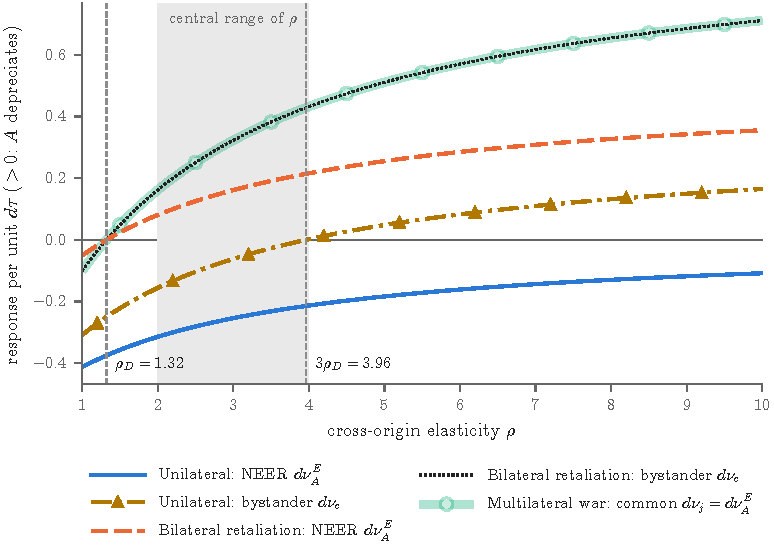
\includegraphics[width=0.8\textwidth]{fig5_configurations.pdf}
\caption{Exchange-rate responses across tariff configurations. Unilateral tariffs, bilateral retaliation, and a multilateral trade war for $N=3$. Retaliation lowers the bystander threshold from $3\rho_D$ to $\rho_D$. \textit{Notes:} US-like calibration; shading denotes $\rho\in[2,4]$.}
\label{fig:configurations}
\end{figure}

\subsection{Preferential tariffs and competing exporters}
\label{sec:pta}

In our model class the bystander's exchange rate is its terms of trade with $A$, $\ToT_{cA}=e_{Ac}$, so the response in \cref{eq:unilateral} is the third-country terms-of-trade effect of a discriminatory tariff, the central object of the preferential-trade-agreement literature since \citet{viner1950} and \citet{mundell1964}. In the canonical competing-exporter model, an importer $A$ that does not produce the good buys it from $B$ and $C$ under quasi-linear preferences. With $q_j$ exporter $j$'s price, $E_j$ its export supply and $M_A$ the importer's demand, a tariff on $B$ always improves $C$'s terms of trade,
\begin{equation*}
\frac{dq_C}{dt_B}=\frac{E'_B}{E'_B+E'_C-M'_A}>0.
\end{equation*}
In our model the bystander gains only if $\rho>N\rho_D$. The difference is that $A$ also produces a competing tradable: part of the demand diverted from $B$ goes to $A$'s own good, along with the rebate's income effect, so the third-country effect survives only when cross-origin substitution is strong relative to domestic diversion. \Cref{app:asym-tariff} shows that at a positive common external tariff the threshold rises, and that a discrete preferential cut requires a higher $\rho$ than the local threshold suggests.
